\chapter{Methodology}
\label{ch:Methodology}
% Most important chapter: talks about my contribution to the topic and what I have achieved

% Goal: Detect ambiguous words in a sentence without context
% 	- Develop method(s) to differentiate from non-ambiguous words: uncover patterns in translation and backtranslation
% 	- Finetune parameters (e.g. how often ambiguous word reoccurs in backtranslation; how many unique words in translation vs. backtranslation)
% 	(-) Suggest alternative translations to ambiguous word
%   (-) Differentiate ambiguous from biased words (cannot say if bias exists or not -> Quality Estimation)

In this chapter, we present the methods used for detecting ambiguity in MT. First, we define the problem around ambiguity that this study attempts to solve. Then, we outline the systematic approach used to solve the problem at hand.

%%%%%%%%%%%%%%%%%%%%%%%%%%%%%%%%%%%%%%%%%%%%%%%%%%%%%%%%%%%%%%%%%%%%%%%%%%%%%%%%%%%%%%%%%%%%
\section{Problem Statement}
\label{sec:Methodology:Problem}

It has been proven that NMT systems reinforce bias present in the training data (e.g., \citet{Prates_2019}, \citet{Stanovsky_2019}). This is typically the case when translating from genderless or notional languages (e.g., English) into grammatical gender languages (e.g., German). One of the most common type of bias is gender bias. 
This bias is often reflected in the way NMT systems translate occupations, since many professions are stereotyped to be either male or female dominated. For example, the occupations "doctor" would often be translated as male, while the occupation "nurse" is most commonly translated as female. 

This study focuses on gender bias, which occurs in consequence of an unresolved ambiguity, meaning that the input text does not contain information regarding the gender of the ambiguous word (e.g., "The \textit{doctor} asked for more information."). More specifically, it attempts to detect patterns in translation which could indicate the presence of an ambiguous word, which is suspected to lead to bias. For this purpose, we make use of existing NMT models based on the Transformer architecture that we described in Section \ref{sec:Background:Transformer}.
 

%%%%%%%%%%%%%%%%%%%%%%%%%%%%%%%%%%%%%%%%%%%%%%%%%%%%%%%%%%%%%%%%%%%%%%%%%%%%%%%%%%%%%%%%%%%%
\section{Approach}
\label{sec:Methodology:Approach}

% Describe the approach in an abstract way

% Input -> Translation -> Backtranslation
In this study, we take a systematic approach to discovering ambiguous words. 

\begin{enumerate}
  \item \textbf{Data Preprocessing:}
  \begin{itemize}
    \item \textbf{Sentence Extraction:} Extract sentences containing an ambiguous word, which we attempt to detect.
    \item \textbf{Replacement:} Generate a new set of sentences replacing the ambiguous word.
  \end{itemize}
  \item \textbf{Translation:} Translate both sets of sentences into the target language.
  \item \textbf{Backtranslation:} Translate the generated translations back into the original language.
  \item \textbf{Evaluation:} Generate statistical results on the translation and backtranslations.
\end{enumerate}

First, we extract sentences containing an ambiguous word, which we attempt to detect. Second, we generate a new set of sentences, replacing the ambiguous word with its disambiguated version or with a common non-ambiguous word. Then, we translate the different sets of sentences into the target language and translate the generated translations back into the original language, also called backtranslating.
Backtranslation means translating a completed translation of the input text back into the original language. The main purpose of the backtranslating technique is to be used for generating statistical results, comparing it with the original text and with its translation. On the basis of these results, we inspect the diversity of the translations and attempt to uncover recurring patterns that could prove an initial assumption. 


% Inter: between two groups
% Intra: within or inside one group
The evaluation of the results happens in two directions:
\begin{itemize}
    \item \textbf{Intra-set Evaluation:} Compare source sentences with target sentences in translation and backtranslation for each set separately.
    \item \textbf{Inter-set Evaluation:} Compare the target sentences in translation and backtranslation of the ambiguous subset with the ones of non-ambiguous subsets.
\end{itemize}


%%%%%%%%%%%%%%%%%%%%%%%%%%%%%%%%%%%%%%%%%%%%%%%%%%%%%%%%%%%%%%%%%%%%%%%%%%%%%%%%%%%%%%%%%%%%
\section{Hypothesis}
\label{sec:Methodology:Hypothesis}
The approach to detecting ambiguous words in text is based on the following hypothesis:

% Main hypothesis (intuition/hypothesis/assumption)
\begin{hyp}\label{main}
Sentences containing an ambiguity produce less diverse backtranslations than sentences without an ambiguity.
\end{hyp}

\setcounter{subhyp}{0}

%%% ??? Translation
% ??? The ambiguous word in a sentence generates more unique words in translation than the corresponding non-ambiguous word.

%%% Backtranslation
% Uniqueness evaluation: sentences
\begin{subhyp}\label{a}
Sentences containing an ambiguous word generate less unique sentences in backtranslations compared to sentences without ambiguous words.
\end{subhyp}

% Uniqueness evaluation: words
\begin{subhyp}\label{b}
Sentences containing an ambiguous word generate less unique words in backtranslations compared to sentences without ambiguous words.
\end{subhyp}

% Alignment evaluation: ambiguous word
\begin{subhyp}\label{c}
The ambiguous word in a sentence generates less unique words in backtranslation than the corresponding non-ambiguous word.
\end{subhyp}

% ??? Alignment evaluation: rest of sentence ???


Fig. \ref{fig:intuition} illustrates the intuition behind the hypothesis. There, the ambiguous word "doctor" is compared against the non-ambiguous version of "doctor", disambiguated with the prefix word "male". The word is first translated into German and the back to English. For each translation direction in the example, two unique translations are generated. In an ideal scenario, the ambiguous word generates the male and female version of the same word in translation, which leads to the same two translation options in backtranslation, while the disambiguated word generates two different words in translation, which are then translated into two other different words. In accordance with the intuition, the ambiguous word has therefore less unique words in backtranslation overall, as depicted in the example.
% propagation of diversity

\begin{figure}
  \centering
  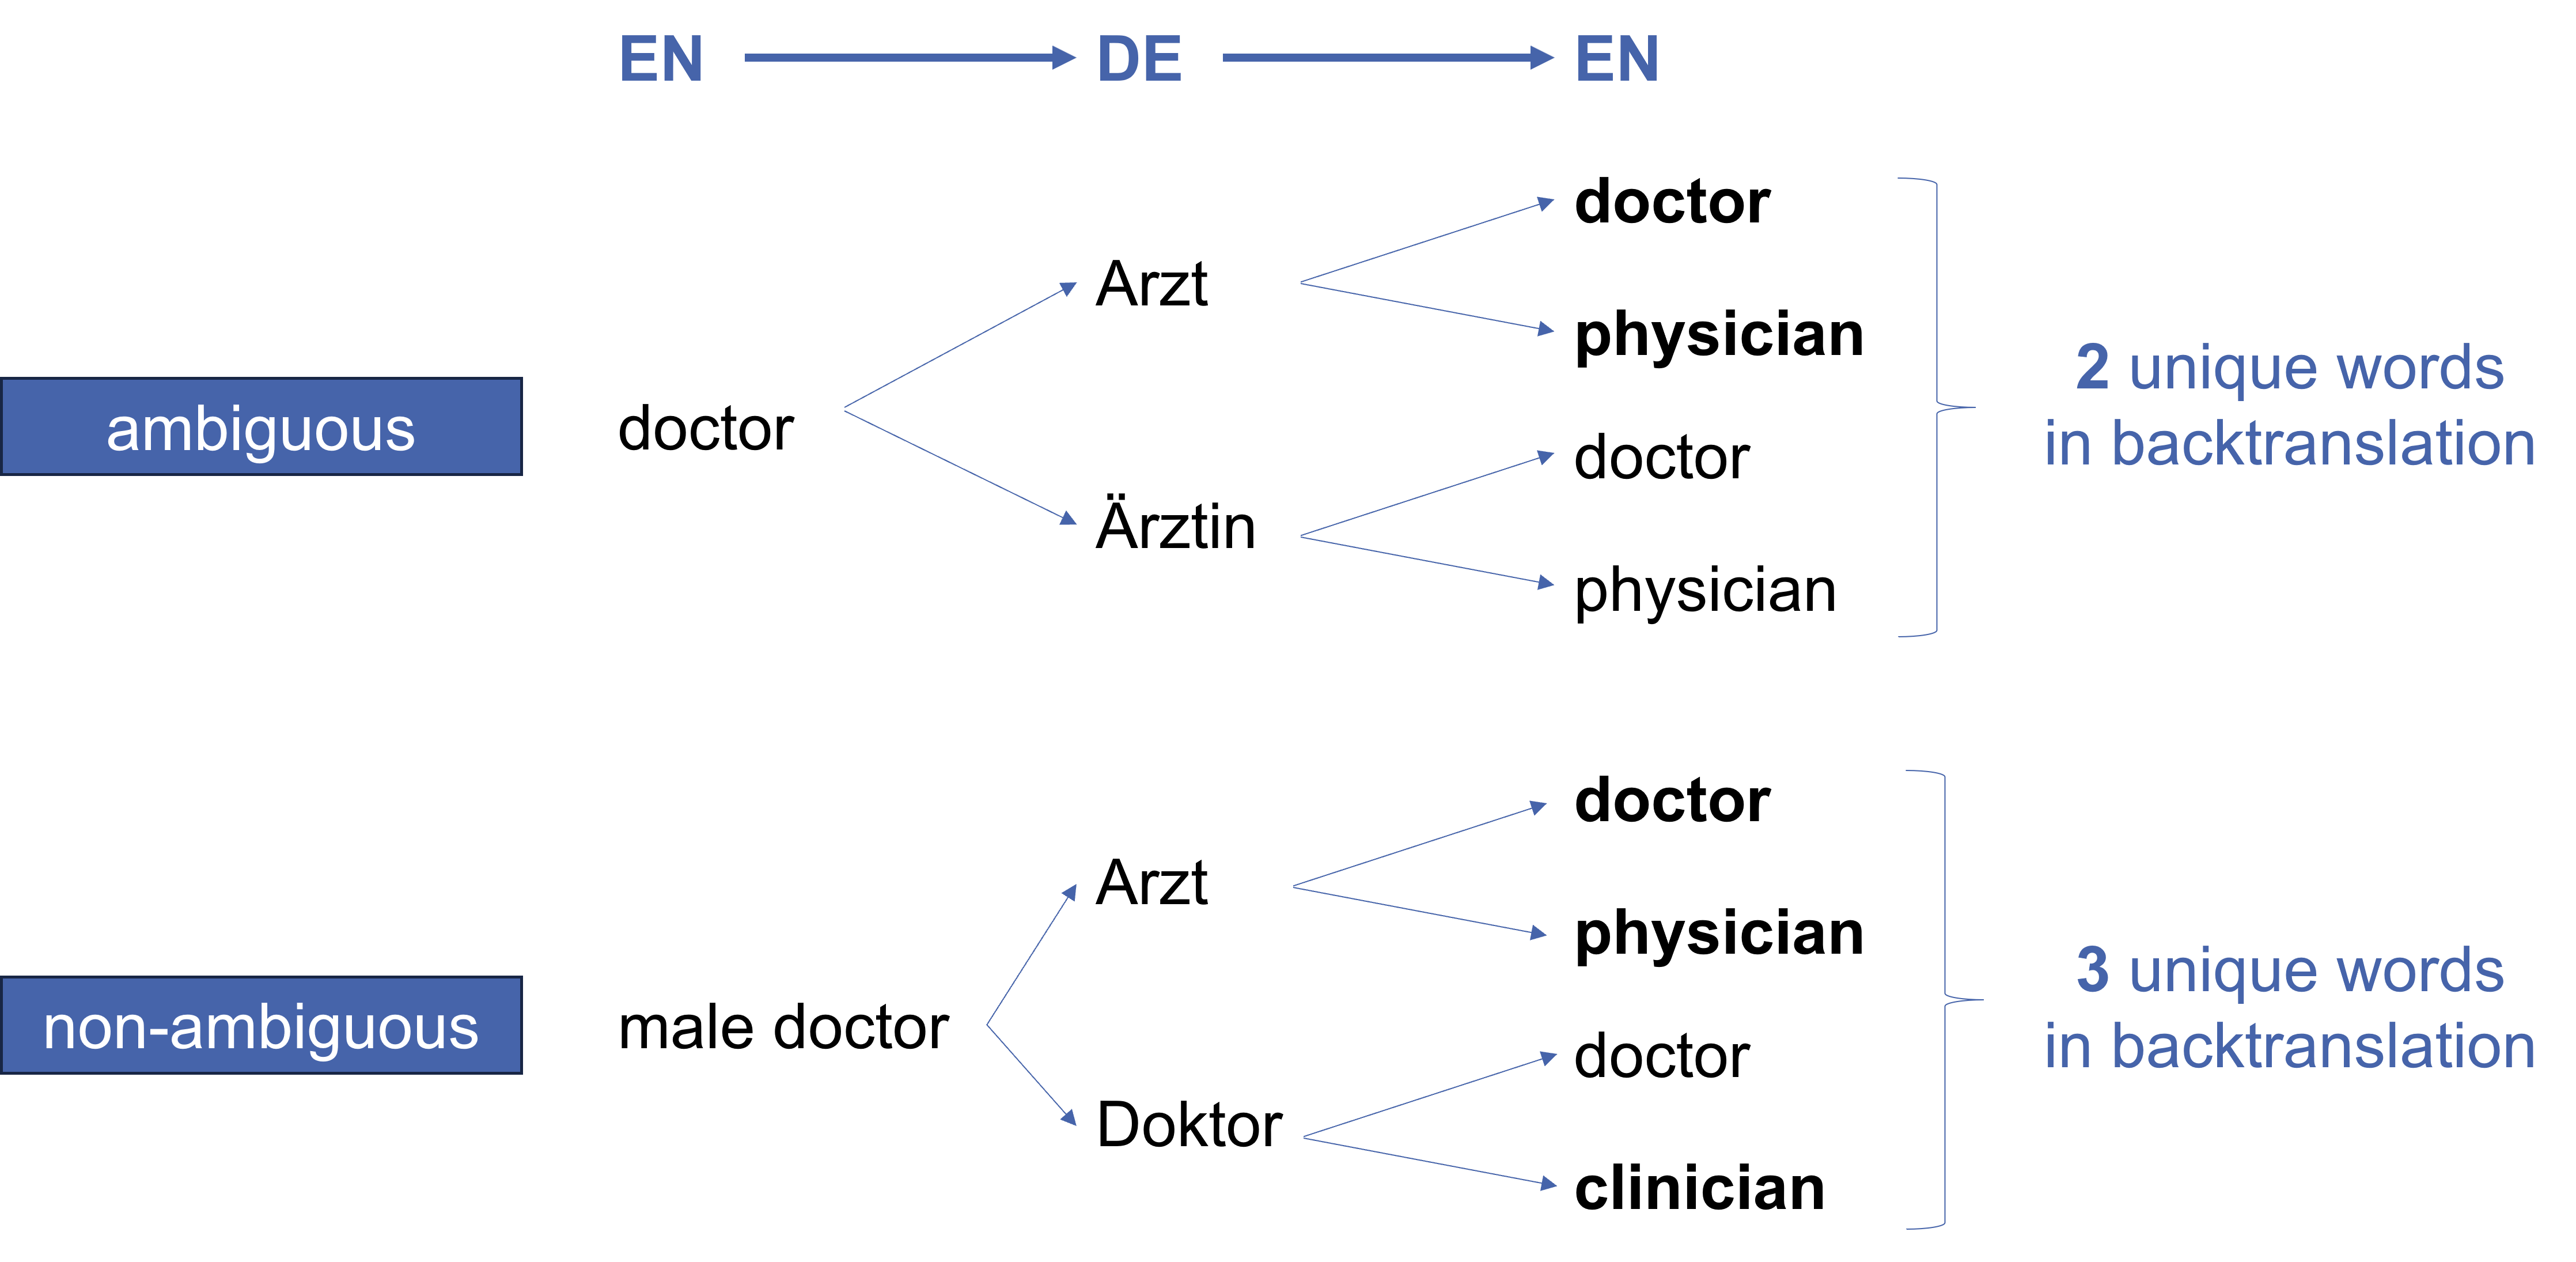
\includegraphics[scale=0.45]{figures/intuition.png}
  \caption{Example Illustration of the Intuition}
  \label{fig:intuition}
\end{figure}

Next, we will perform a more thorough explanation of the different experimental conditions and steps followed to inspect the assumption.



